\documentclass[12pt]{article}

\usepackage{url}
\usepackage{graphicx}

% This makes paragraphs with titles start on a new line
\makeatletter
\renewcommand\paragraph{\@startsection{paragraph}{4}{\z@}%
  {-3.25ex\@plus -1ex \@minus -.2ex}%
  {1.5ex \@plus .2ex}%
  {\normalfont\normalsize\bfseries}}
\makeatother

\title{G52GRP Interim Group Report}                     % used by \maketitle
\author{gp09-jqg\thanks{Dhruv Gairola, Chris Head, Rob Miles, Amy Jane Wesson and Chenjue Xu, supervised by Julie Greensmith}} % Alphabetical order
\date{November 30, 2009}                                    % used by \maketitle

\setlength{\topmargin}{-.4in}
\setlength{\textheight}{9in}
\setlength{\oddsidemargin}{.125in}
\setlength{\textwidth}{6.25in}

\begin{document}
\maketitle                                              % automatic title!

\tableofcontents
\newpage

\section{An Introduction to the ``Problem''}
\begin{figure}
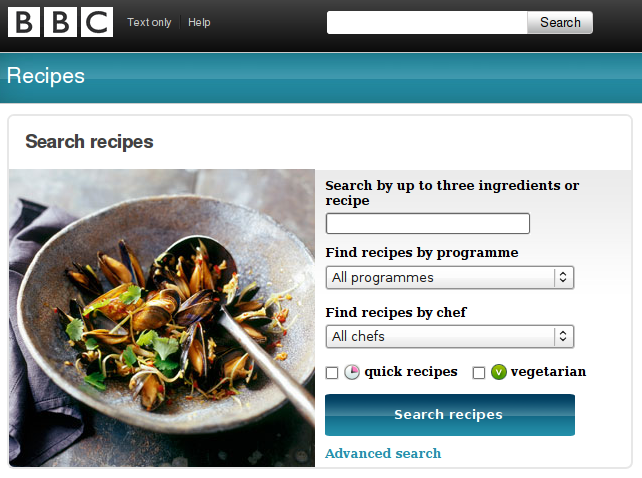
\includegraphics[width=0.9\textwidth]{screenshot_bbc_recipes}
\caption{The BBC Food Recipe Search Page}
\label{fig:bbc_food}
\end{figure}

The aim of this project is to develop a software kitchen assistant tool. This tool must be able to provide recipes which match a supplied list of available ingredients. This is similar to the BBC's recipe search\footnote{\url{http://www.bbc.co.uk/food/recipes/}} (Fig~\ref{fig:bbc_food}), but is not constrained to just three search items. The software should, in essence, provide recipe matches to help the user make recipe decisions given the ingredients he/she currently has. This involves making recommendations and provides us with an avenue to make use of collaborative filtering technology. Additionally, the recipe database can be community maintained, and aspects of social networking can be implemented to encourage user participation. The main draw of the project lies in its inherent flexibility, which extends from the plethora of expansion decisions which can be made to enhance user experience.

\newpage

\section{Product Specification} 			%Product Spec
In response to our initial meeting with our client and after reviewing the ''Problem Description'', we have put together a brief specification stating the requirements for the software at three levels which have been agreed by our client. The levels can be considered as versions as they will be implemented in this way (i.e. Minimum - version 1.0, Realistic Best -  version 2.0 and Ideal - version3.0 \footnote{It should be noted that due to the nature of creating a solution there are likely to be intermediate versions e.g. 1.2, which will be used solely in the repository.}). These requirements will be used as a basis for the design of the respective versions and the designs will be created with these requirements in mind.

\subsection{Minimum - v1.0}

The requirements listed below are the minimum requirements to make the software work which does not include extra functionality desired by our client. This will be the Version 1.0 of our prototype and we will use this as a base to build from. 
Furthermore, the creation of different versions with the intent to expand on previous versions will allow for continuity between languages and eliminating the need to 'start from scratch'.

\begin{itemize}
	\item Contains several recipes in a database.
	\item Has a Web Interface.
	\item Recipes are searchable by ingredients (greater than 3 ingredients).

\end{itemize}

\subsection{Realistic Best - v2.0}

The requirements below are what we have identified as the most realistic outcome of the software within the time constraints. This would meet all the minimum requirements outlined by the client and some desirable ones as well. This will
essentially be an expanded/upgraded version 1.0 .

\begin{itemize}
	\item Has a large database of recipes.
	\item Has a clean, attractive web interface.
	\item Has a seperate, simpler web interface for mobile devices.
	\item Recipes are searchable by combinations of ingredients.
	\item Has user accounts.
	\item Allows users to rate recipes.
	\item Gives recipe recommendations based on past ratings.
\end{itemize}

\subsection{Ideal - v3.0}

Below are the requirements for the software if it were to be the ideal solution to the problem. This list includes existing requirements from v1.0 and v2.0 at a higher level and all desirable requirements as well. It is likely that only few of these requirements will be fulfilled in the final version that is submitted. 

\begin{itemize}
	\item Has a very large, automatically updated and maintained database of recipes.
	\item Has a clean, attractive and user-friendly web interface.
	\item Has a mobile device optimised interface and an iPhone application.
	\item Recipes are searchable by combinations of ingredients.
	\item Recipes are searchable by other tags: 'vegetarian', 'italian', 'low fat' etc.
	\item Has a full user system with profiles and user-uploaded recipes.
	\item Supports social media functions.
	\item Allows users to rate, tag and commment on recipes.
	\item Gives recipe recommendations based on past ratings and accumulated data from the entire user base.
	\item Gives recipe recommendations for several users i.e. 'A recipe that Alice and Bob both like'.

\end{itemize}

\newpage


\section{Results of Technical Research}		%new section on research

For this part of the project we looked into many different alternatives for suitable platforms,
tools, technologies, algorithms and data structures. We mainly conducted our research using the internet however, 
we did use some of our own personal experience and preferences aswell to influence our decisions.

\subsection{Platform Decisions}

\paragraph{Microsoft Windows}
The windows operating systems have long dominated the operating system industry. Approximately 90 \% of users use Windows operating systems, chiefly Windows XP followed by Windows Vista. Its ease of use and engaging graphical interface is certainly an attraction. However, precisely due to its widespread usage, Windows is the prime target for malware. Microsoft however, does provide bug fixes and other help to stabalise the system. Moreover, most forms of software run on Windows.

If our group is to market our product to customers, it makes sense that we focus on Windows as the platform of choice since it is the most commonly used operating system. Moreover, if our project decides to make an application, it should be able to run in Windows, and since most software works on Windows, it is the clear choice.

\paragraph{Mac OSX}
Although not as widely used as Windows, this operating system has a very encouraging user interface which is easy to pick up. It is claimed as being more secure than Windows, due to its UNIX base. However, recent reports suggest the Apple’s Snow Leopard system is less secure compared to Windows Vista and XP\footnote{ [ http://www.wired.com/gadgetlab/2009/09/security-snow-leopard/ ].}. Of course we must take into account the comparatively fewer threats from malware on Mac OSX. 
Mac OSX also uses pre-emptive multitasking for all native applications to which decreases the incidence of multiple program crashes.

\paragraph{Linux}
One of the biggest advantages of Linux over other operating systems is the Linux kernel which ensures a basic level of security. Its hardware requirements are also much lesser than Windows and Mac OSX. Additionally, Linux, being open source is a free system. Linux distributions like Ubuntu, also provide a friendly and graphical user interface for users to work with. However, latest hardware is typically slower to reach linux. Moreover, depending on the distribution, the learning curve of Linux might be daunting for users \footnote{[ http://packratstudios.com/index.php/2008/04/06/the-pros-and-cons-of-linux-windows-and-osx/ ]}.

\subsection{Technologies}

\paragraph{Django}
A web framework based on Python language, Django is relatively easy to understand, Python being easier to program due to its natural language-like syntax. One of chief arguments for the use of Django concerned software reuse. Various existing libraries can be used to aid our software development efforts. The group software head also backed Django, and his recommendation was well received since the group could learn a new form of technology while benefiting from his expertise.
\begin{itemize}
\item Advantages
	\begin{itemize}
	\item Our Technical Officer has experience developing with Django which is beneficial when developing and learning the language.
	\item Python is an easy language to learn and use, with a focus on simplicity and ease of use whilst providing an elegant solution to the problem.
	\item A variety of third party plugins coincide with our site's functionality, saving a lot of work by maximising code reuse.
	\end{itemize}
\item Disadvantages
	\begin{itemize}
	\item Requires learning a new language.
	\end{itemize}
\end{itemize}


\paragraph{Ruby on Rails}
A web framework based on Ruby language, it allows users to create powerful applications using simple coding without compromising on the functionality of powerful languages\footnote{[ http://www.hosting.com/support/rubyonrails/faq/ ]}. The Rails framework also has many pre-defined libraries and functions that we may be able to use to our advantage.
\begin{itemize}
\item Advantages
	\begin{itemize}
	\item Increased code reuse due to vast array of pre-defined libraries and functions available.
	\item Also provides an esay and elegant solution to complex web programming problems.
	\end {itemize}
\item Disadvantages
	\begin{itemize}
	\item Abstraction may mean sacrificing fine control even when it would be useful.
	\item None of our group are familiar with the Ruby framework which may affect our pre-defined timetable and/or our time constraints.
	\end {itemize}
\end {itemize}

\paragraph{PHP with SQL}
This option was an attractive one, considering that members had some experience with PHP and SQL previously. Moreover Java, Python, C++, Ruby are normally used to create complex systems which is not necessary for us 
at this stage in the project.
\begin{itemize}
\item Advantages
	\begin{itemize}
	\item Overall group experience with these languages. 
	\item Common technology means it is well supported with many tutorials and guides on usage.
	\end {itemize}
\item Disadvantages
	\begin{itemize}
	\item Low level control means making large systems is complicated and difficult.
	\end {itemize}
\end {itemize}

\paragraph{Web Browser Options}
In theory, all web browsers are the same, and any page that works on one will work on all others, as long as they all support the same standards. In practice this is not the case and different browsers support different features. The main browsers right now are Microsoft Internet Explorer, Mozilla Firefox, Safari, Google Chrome and Opera\footnote{\url{http://www.w3schools.com/browsers/browsers_stats.asp}}. Of these, the majority support the web standards codified by the World Wide Web Consortium (W3C)\footnote{\url{http;//www.w3.org}}, so in order to easily gain compatibility with the largest number of web browsers, we will aim to write a W3C standard compliant site. We can test this with W3C's validator\footnote{\url{http://validator.w3.org/}}, which will save us having to debug the site in every browser we wish to support






























\newpage

\section{Implementation Options}
\subsection{Summary of Project Description and Specification}

The project description implies the implementation of some form of a database, either online (i.e. on a website) or offline (i.e. run on a local machine as an executable program). There are no specific details as to which language, layout or structure etc, are to be used when creating the solution. There are also no details as to which Operating System the solution should be created for and whether additional software/hardware is allowed. Considering this we have ‘taken it open ourselves’ to discuss and choose what we thought was a suitable target platform and have also discussed availability of software/hardware needed to create the solution.
During an initial meeting with our client concerning the problem specification/requirements it has become clear that the preferred solution is to create a website with a database backbone. This can be implemented in many different styles/languages which we have also discussed extensively.
 
We have created the Problem Specification (section~\ref{sec:productspec} on page~\pageref{sec:productspec})
% You can stick labels to sections and have it update the page number if it changes!
 with the intent that at each stage, the structure and format of the solution allows successive stages to be completed without changing the entire structure too much. This prototyping adheres to a large extent with the concept of Extreme Programming, where frequent releases introduce checkpoints where new customer requirements can be adopted. Additionally, the focus will be on upgrading versions of prototypes. To accommodate this dynamic character of our project, we need a framework which ties in the database with all the different elements of the website.


\newpage

\section{Initial design of the proposed system and its user interface}
The version 1 website colour scheme is an amalgamation of white (for the background) and orange (for miscellaneous design features). The white background leverages on its simplicity and clarity, an important criteria for retaining the attention of the user. Moreover, the orange colour is reportedly stimulating for the users appetite\footnote{[ http://desktoppub.about.com/cs/colorselection/p/orange.htm ]}. The group also agreed on an orange logo design. 

\subsection{Version 1}

\begin{figure}[h]
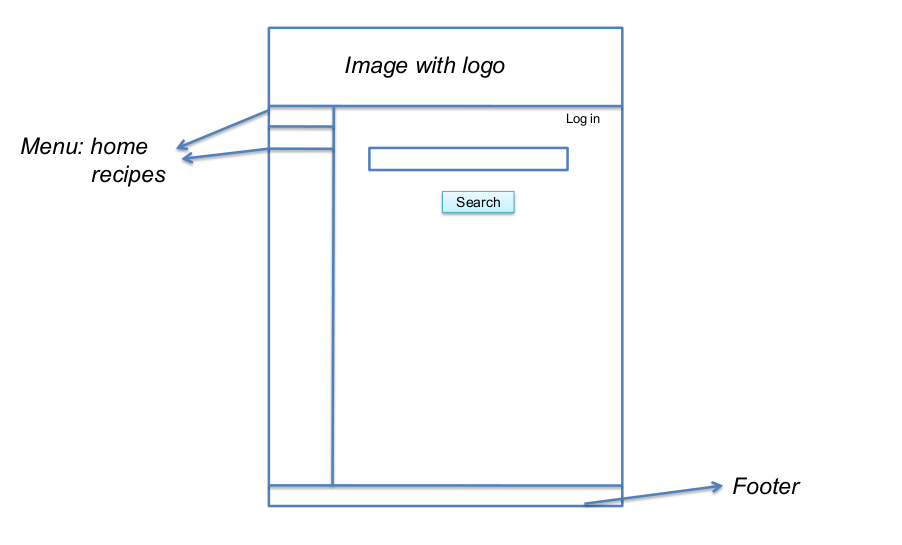
\includegraphics[width=0.9\textwidth]{home_page}
\caption{Layout of the Home Page}
\label{fig:home_page}
\end{figure}

The merit of the version 1 website design is in its simplicity. Upon accessing the website, (Fig~\ref{fig:home_page}) users are presented there are three drop-down menus which allows people to select ingredients. The drop-down menus are transversely positioned to accommodate the vertical cascading of the ingredients of the menus. Users are provided with three menus to select ingredients and submit a search. This then links to the recipe list page. Additionally, the “recipes” button in the sidebar links the page to the complete list of recipes alphabetically.

\begin{figure}[H] % Place it [H]ere, you big furry oaf! I don't care what you smell! 
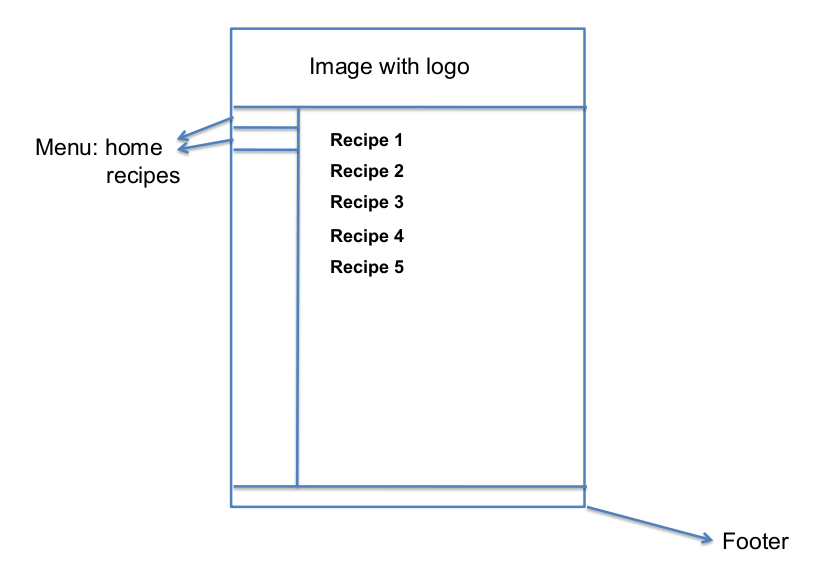
\includegraphics[width=0.9\textwidth]{recipe_list_page}
\caption{Layout of the Recipe List Page}
\label{fig:recipe_list}
\end{figure}

The recipe list page (Fig~\ref{fig:recipe_list}) contains a list of recipes with at least one of the three ingredients. However, the recipe may contain other ingredients which were not specified by the user. Upon recipe selection, the specific recipe page will be displayed.

\begin{figure}[H]
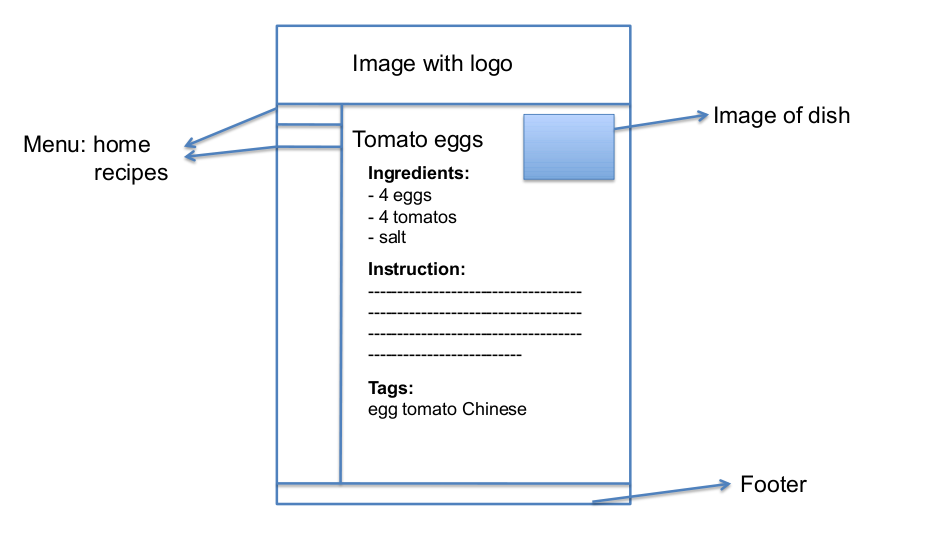
\includegraphics[width=0.9\textwidth]{recipe_page}
\caption{Layout of the Recipe Page}
\label{fig:recipe_page}
\end{figure}

The recipe page (Fig \ref{fig:recipe_page}) contains recipe details, for example recipe name, ingredients, the instruction, and recipe tags.
 
One design limitation of version 1 is that the website only has three drop-down menus, and the user is unable to type in ingredients. Being a prototype, the version 1 database is fitted with few recipes hence such functionality is redundant. 

\subsection{Version 2}
Version 2 is an upgraded version of the original version containing more functions (described by the Product Specification). With the use of technology such as JAVA Script, the web interface will look more polished. Users will be able to enter text data into ingredient selection text boxes, which will have the tab completion feature for ingredients instead of using a drop-down menu. There will also be a larger database of ingredients hence justifying the use of tab completion as apposed to drop-down menus.

Additionally, for version 2, users are allowed to have web accounts. The benefits of the account include the user having access to past recipes which he/she rated and more importantly receive recommendations of recipes they might like (this uses collaborative filtering technology). In addition, users could choose to click tags and get a list of recipes that contains that particular tag.

Additional website link may likely be created, for example a link to the most popular recipes. The website is also expected to be optimised for mobile phone viewing.

\subsection{Version 3}
The ideal version of our product involves the implementation of a variety of possible functionalities. For example, a mobile application could be developed. Recipes could be made searchable by not just ingredients but also, for instance, the type of cuisine (Chinese dish) or whether recipes are vegetarian or non-vegetarian. 

Social networking is another possibility, with users being able to interact with other users and leave comments of the pages of other users. Users might be able to upload their own recipes and receive ratings from other users. The possibility for improvements are abundant.

\newpage

\section{Implementation Decisions}

\subsection{Decision Influences}

\subsubsection{Aims}

The aims of version 1 have a strong influence over implementation decisions. They are as follows;

\begin{enumerate}
\item To be a complete working release of a usable piece of software
\item To allow the team to familiarise themselves with the tools and systems to be used for later versions
\item To explore the capabilities of those systems, to inform and inspire later decisions.
\end{enumerate}


\subsubsection{Design Principles}

The project is being developed using a version of the Extreme Programming (XP) Methodology. XP's software development principles have an impact on the software design principles of projects developed using it.

Similarly the Web Framework Django has its own set of design philosophies\footnote{\url{http://docs.djangoproject.com/en/dev/misc/design-philosophies/}} which also influence the project's design principles.

The principles of XP and Django are quite similar and complement one another quite well, so it is possible to abide by both sets of principles without contradictions.

Some of the XP/Django principles that have the most influence on implementation decisions are listed below;

\begin{description}
\item[DRY] Don't Repeat Yourself \\
Every piece of knowledge must have a single, unambiguous, authoritative representation within a system.
\item[YAGNI] You Aren't Gonna Need It \\
Always implement things when you \textit{actually} need them, never when you just \textit{foresee} that you need them
\item[Maximise Code Reuse] If two bits of code look similar, move them out into a more general function. If two functions do a similar thing, merge them. This keeps redundancy low.
\end{description}

Both XP and Django have a strong basis in philosophy and principles, and while they both leave the developer the freedom to chose their implementation decisions, they are designed to work best with implementations that follow their principles.

\subsection{Decisions}

\subsubsection{The \texttt{recipes} App}

Recipes are the only thing that version 1 does, so it would make some sense to simply have the project as a whole perform the recipe functions, and not use any apps. However, the functionality of the site was put in a \texttt{recipes} app for two reasons.
Firstly, it is best practice in Django to have all code in conceptually distinct, reusable apps, to maximise potential code reuse.
Secondly, as one of the aims of this version is to introduce the team to working with Django, and apps are a major part of Django, it made sense to use apps even if they are not strictly necessary.


\subsubsection{URL Design}

The URL design is intended to be very simple and readable. In accordance with Django URL design principles, there are no filename extensions in URLs.


\subsubsection{Model Design}

The only implementation decision of note in the model design is the use of a python \texttt{property} to handle recipe tags. A \texttt{property} is a python language construct that behaves as though it is a class variable, but behind the scenes calls a getter or setter function when it is fetched or assigned to. This was used because, although it makes the model less readable, it makes all of the code that deals with the model far more readable, and it is this code which is more complex and benefits more from simplification.

\subsubsection{View Design}

\paragraph{The \texttt{recipe\_list} View}

There are 2 views that simply show a list of recipes:- \texttt{recipes\_all} (the view of all recipes on the system) and the results section of \texttt{search} (the view of all recipes that meet the search terms). In order to maximise code reuse, the functionality of displaying a list of recipes was taken out into a separate \texttt{recipe\_list} view, which is called by both \texttt{recipes\_all} and \texttt{search}.

\paragraph{The \texttt{search} View}

The search is deliberately the simplest search possible that meets the specifications. The set of results is simply the set of recipes which contain any of the ingredients searched for. This will be radically improved in later releases.

\subsubsection{Template Design}

\begin{samepage}
\begin{quote}
``The most powerful -- and thus the most complex -- part of Django's template engine is template inheritance. Template inheritance allows you to build a base ``skeleton" template that contains all the common elements of your site and defines blocks that child templates can override."\flushright-- Django's Template Documentation\footnote{\url{http://docs.djangoproject.com/en/dev/topics/templates/}}
\end{quote}
\end{samepage}

\noindent Template Inheritance provides a good opportunity to maximise code reuse, but it was not used in version 1 in an attempt to keep template design simple.














\newpage

\section{Research} %quite aware this is in the wrong place, idk where the right place is
\subsection{BBC Recipes}

\begin{figure}
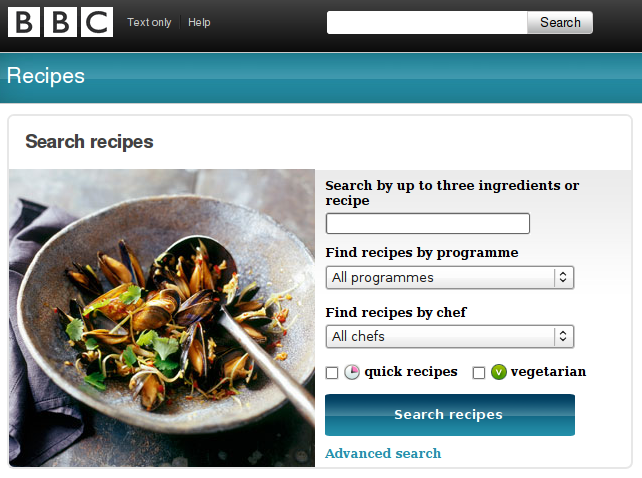
\includegraphics[width=0.9\textwidth]{screenshot_bbc_recipes}
\caption{The BBC Food Recipe Search Page}
\label{fig:bbc_food}
\end{figure}


BBC Recipes (Fig~\ref{fig:bbc_food}) is a web application that allows the user to input up to three ingredients and returns a list of related recipes. 

BBC Recipes has two search options, basic and advanced. The basic search allows the user to input up to three ingredients with the option to find the recipe by television program or by chef. This search also provides the tagging options of quick recipes and vegetarian. However the advanced recipe search includes a wider choice of search preferences such as, the preparation method, cuisine, season and dietary requirements. After looking over the source code it’s very obvious that this web-based application uses an online database using a query language to return recipe results. 

One main advantage about this application is the advanced search option which includes a numerous amount of tag options. This option becomes quite useful when searching through a large database as this kind of search minimizes the results. A good example of this is a search including flour, butter and sugar with the season tag being ‘Christmas’ and the dietary needs tag being ‘nut-free’ returning only 14 recipes. However a search including just the three ingredients returns 400 recipes. 

One flaw that I have noticed with the search is that the search field is a text box which involves text input, this not validating the input until creating the search. The validation matches the input with similar words, for example for ‘flor’ it will return ‘flour’. However when having typo’s like ‘aooples’, instead of ‘apples’ the returned match is ‘allows’. To solve this issue a drop-down menu including the ingredients from the database would perhaps be a better idea.

The design of the website is attractive with a good use of colour and images. However the navigation of the website is slightly tedious, the reason for this being when expanding the actual recipes on the home page the webpage’s content increases and therefore leaving the user to have to scroll through the webpage to view it’s content. 



\subsection{RecipeZaar.com}

\begin{figure}
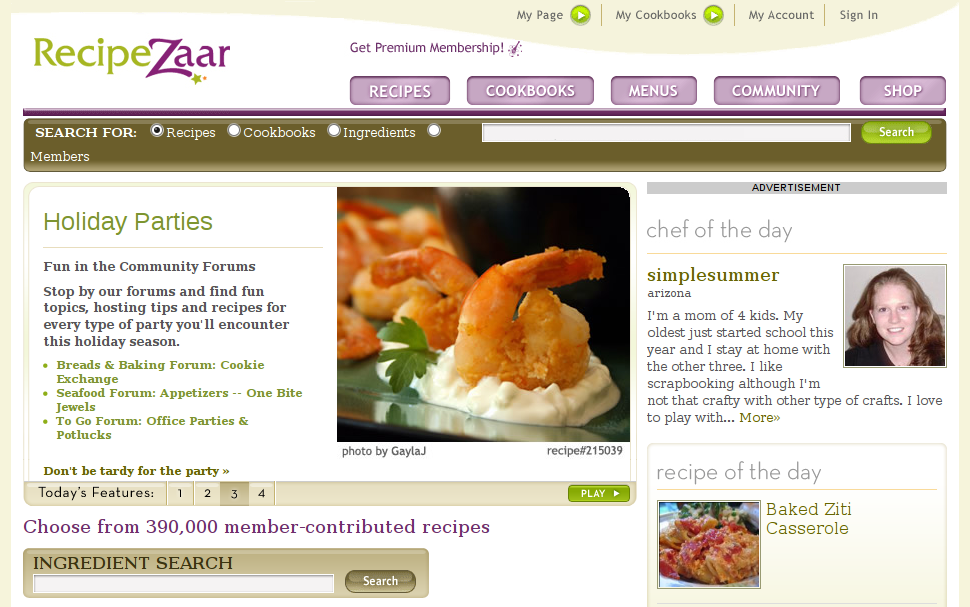
\includegraphics[width=0.9\textwidth]{screenshot_recipezaar}
\caption{The RecipeZaar.com Home Page}
\label{fig:recipezaar}
\end{figure}

Recipezaar (Fig~\ref{fig:recipezaar}) is a website that includes a large database of recipes and user accounts. Recipes are searchable by recipes, cookbooks, ingredients and members. 

The recipe search allows the user to input n number of ingredients. The input method is a text box which includes no validation. If the user inputs ‘flor’ instead of ‘flour’ the search returns nothing. The query used for this search seems to be very basic, the reason for this being if the user inputs ‘flour, sugar, butter, eggs’ for example one of the returned recipes is ‘vegetable casserole’ which doesn’t contain any of the above ingredients. Another example of a recipe is ‘leach family turkey stuffing’ which only contains one of the above ingredients. Because the search isn’t specific and because the website has a large online database the results are too vague.

This website introduces the use of collaborative filtering by including user accounts with the option to upload recipes and rate other recipes. When viewing a member’s recipe theres also the option to send a private message, submit corrections, send the recipe to the users email address or mobile device and create a shopping list. The recipe page also directs the user to other recipes ‘like’ the chosen recipe. The website also has a community webpage with forums for general discussions. 

The design of the website is interactive with a good use of JavaScript. The colour scheme is neutral with a good use of images.




\newpage

\section{Expanded Problem Description}
As a group we understood that the aim of the project is to develop a software kitchen assistant tool. The tool must be able to provide recipes which match a supplied list of available ingredients. The software should provide a number of matching recipes and rank the suggestions according to how well they match. The database will also take into account user’s own food preferences, this allows us to introduce collaborative filtering technology to manage the recommendations. 

We have chosen to use extreme programming therefore making frequent and small releases. We have specified three versions, these being minimum, realistic and ideal. 

For all three versions the interface of the kitchen assistant tool will be web-based and will allow the user to select at the least three ingredients. Once these ingredients are submitted it will return a list of recipes that are ranked in accordance to how well the recipe matches the selected ingredients. 

Version 1 will be a web-based application with a simple interface using only HTML, CSS and Django template markup. The online database will contain several recipes that are searchable by ingredients.

Version 2 is an extended version of v1.  The web-based interface will introduce JavaScript, AJAX (asynchronous JavaScript and XML) and JSON (JavaScript Object Notation). The online database for this version will contain a vast amount of recipes that are searchable by a combination of ingredients. With the introduction of collaborative filtering we intend to create user accounts that allows the user to rate recipes and then return recommendations based on previous ratings. 

Version 3 extends v2. The web-based interface will remain the same however we will create a mobile optimised interface and an Iphone application. The online database for this version will include a very large amount of recipes that are automatically updated and maintained. Recipes will be searchable by combinations of ingredients and by other tags such as ‘vegetarian’, ‘Italian’, ‘low fat’, etc. Returned recipes will be returned based on past ratings and accumulated data from the entire database. Recipes will also give recommendations for several users i.e. ‘A recipe that alice and bob will both like’. This version will include a full user system with profiles and user-uploaded recipes. The application will support social media functions such as messenger, the possibility of rating, tagging and commenting on other recipes. 

The project has be divided into 5 managerial area’s. These being management, technical, design, quality assurance and documentation. Every member has been given the responsibility of one of these areas and is expected to ensure all targets are met.




\end{document}             % End of document.
